\documentclass[a4paper,12pt]{article} 

%Das Paket wird für die anderthalb-zeiligen Zeilenabstand benötigt
\usepackage{setspace}
%%%%%%%%%%%%%%%%%%%%%%%%%%%%%%%%%%%%%%%%%%%%%%%%%%%%%%%%%%%%%%%%%%%%%%%%%%%%%%%%%%%%%%
%%                                                                                  %%
%% HTWM-Vorlage - benoetigt folgende Pakete:                                        %%
%% apt-get install texworks texlive-fonts-extra kile kile-l10n aspell-de texlive-lang-german  %%
%%                                                                                  %%
%% empfohlener Editor: TexWorks                                                     %%
%% %%%%%%%%%%%%%%%%%%%%%%%%%%%%%%%%%%%%%%%%%%%%%%%%%%%%%%%%%%%%%%%%%%%%%%%%%%%%%%%%%%%
\setcounter{tocdepth}{3}			%Schatelungstiefe Inhaltsverz.
\usepackage[utf8]{inputenc}			%deutsche Umlaute
\usepackage{german, ngerman}
\usepackage[ngerman]{babel}			%Rechtschreibprüfung
\usepackage{color,listings} 			%Quellcode Highlighting, bindet das
%Paket Listings ein
\usepackage{listings}
\usepackage{pdflscape}
\usepackage{color}
\usepackage{textcomp}
\usepackage{float}
\usepackage[T1]{fontenc}			%srccode
\usepackage[scaled]{beramono}			%srccode
\usepackage{longtable}				%mehrseitige Tabellen
\usepackage[tableposition=b]{caption}
\usepackage[pdftex, pdftoolbar=false, hyperfootnotes=false, bookmarks,
bookmarksopen, bookmarksnumbered, bookmarksopenlevel=2, pdfpagelabels=true,
pdfstartpage=3, pdfstartview=FitH,]{hyperref} %Verlinkungen
\usepackage{array}				%farbige Tabellen
\usepackage[table]{xcolor} 			%farbige Tabellen
\usepackage{graphicx}				% \includegraphics bnoetigt dies

\usepackage{fancyhdr, graphicx}			%% Logo auf Titelseite

\usepackage{amsmath,lipsum}		%% mathematisches +-

\renewcommand{\headrulewidth}{0pt}
\fancyhead[L]{}
\fancyhead[R]{
%  \includegraphics[width=52mm]{./images/htwk.png}
}
%\usepackage{draftwatermark}			% wasserzeichen
%Quelle: http://choorucode.com/2010/05/05/latex-adding-draft-watermark/?like=1&source=post_flair&_wpnonce=1c9f85538d
%\SetWatermarkText{VORABVERSION}		% wasserzeichen-text
%\SetWatermarkLightness{0.9}			% wasserzeichen-kontrast
%\SetWatermarkScale{2.5}				% wasserzeichen-zeichengroe\ss{}e

\definecolor{Navy}{rgb}{0,0,0.5}
\definecolor{Gray}{gray}{0.5}
\definecolor{dunkelgrau}{rgb}{0.8,0.8,0.8}
\definecolor{hellgrau}{rgb}{0.95,0.95,0.95}
\definecolor{hellgrau2}{rgb}{0.93,0.93,0.93}

\hypersetup{
	colorlinks=true, 			% false: boxed links; true: colored links
	linkcolor=Navy,          		% color of internal links
	citecolor=Gray,        			% color of links to bibliography
	filecolor=magenta,      		% color of file links
	urlcolor=blue,           			% color of external links
	linkbordercolor={1 1 1}, 		% set to white
	citebordercolor={1 1 1} 		% set to white
}


%Einrückung eines neuen Absatzes
%\setlength{\parindent}{0em}

%Definition der Ränder
\usepackage[paper=a4paper,left=30mm,right=30mm,top=30mm,bottom=30mm]{geometry}

%Abstand der Fussnoten
%\deffootnote{1em}{1em}{\textsuperscript{\thefootnotemark\ }}

%Regeln, bis zu welcher Tiefe (section,subsection,subsubsection) Überschriften angezeigt werden sollen (Anzeige der Überschriften im Verzeichnis / Anzeige der Nummerierung)
%\setcounter{tocdepth}{3}
%\setcounter{secnumdepth}{3}

%%%% HTWK-Logo rechts oben einfuegen funktioniert nicht :/
%\fancypagestyle{htwkheader}
%{
%   \fancyhf{}	% clear all header and footer fields
%  \fancyhead[RO]{
%	\makebox[\textwidth]{	%% schiebe Logo nach aussen auf den Rand
%		\rule{1				%% nach aussen schieben hoeherer Wert -> Logo weiter nach aussen
%		  \textwidth}{0cm} %% nicht nach unten schieben = 0cm
%			\includegraphics*[width=52mm]{./images/htwk.png}	%%Logo HTWK
%	  }
%  }
%}

%%bibliography setting
\bibliographystyle{alpha}

\begin{document}
 
%Beginn der Titelseite
\begin{titlepage}

\begin{small}
\begin{flushleft}
\vfill {
HTWK Leipzig\\
Fachbereich IMN \\
Sommersemester 2014}
\end{flushleft}
\end{small}
 \begin{verbatim}












\end{verbatim}
\begin{center}
\begin{Large}
\textsf{\textbf{
SmartCard-Projekt SS 2014\\
Traincard\\
}}
\end{Large}
\end{center}
\begin{verbatim}












\end{verbatim}
\begin{flushleft}
\begin{tabular}{lll}
\textbf{Thema:} & & Erstellung eines On- und Offcard Programm,\\
& & welches eine JCOP fähige Smartcard befähigt,\\
& & intelligent zwischen Fitnesstrainer und Sportler\\
& & zu agieren.\\
& & \\
& & \\
\textbf{eingereicht von:} & & Kurt Junghanns, B.Sc.\\
& & Marcel Kirbst, B.Sc.\\
& & Michael Reher, B.Sc.\\
& & \\
& & \\
\textbf{Datum:} & & \today\\
& & \\
& & \\
\textbf{Betreuer:} & & Prof. Dr. rer. nat. Uwe Petermann\\
\end{tabular}
\end{flushleft} 

\end{titlepage}
%Ende der Titelseite

\newpage
\pagenumbering{Roman}
\setcounter{page}{1} 
%Inhaltsverzeichnis (aktualisiert sich erst nach dem zweiten Setzen)
%\addcontentsline{toc}{chapter}{Inhaltsverzeichnis}
%\tableofcontents


% Abbildungsverzeichnis
%\newpage
%\addcontentsline{toc}{chapter}{Abbildungsverzeichnisverzeichnis}
%\listoffigures

% Listingverzeichnis
%\newpage
%\addcontentsline{toc}{chapter}{Listingverzeichnis}
%\lstlistoflistings
 
%Beginn einer neuen Seite
\clearpage
 
%Anderthalbzeiliger Zeilenabstand ab hier
\onehalfspacing

%Eine Zeile Abstand nach jedem Absatz und 1,5 er abstand nach jeder zeile
%\renewcommand{\baselinestretch}{1.5}\normalsize
\setlength{\parindent}{0pt}
\setlength{\parskip}{8pt}
%\sloppy
 
%%\pagestyle{plain}
 
\newpage
\pagenumbering{arabic}
\setcounter{page}{1} 
%% Inhalt


%% Nicht vergessen: wir sollen "behandelte" Techniken verwenden und die Verwendung hier anpreisen

\section{Use-Case}
Dieses Projekt richtet sich an Sportler und ihre Trainer.

Jeder Sportler erhält eine persönliche Smartcard, womit er Zugriff auf seinen Trainingsplan hat und seinen Fortschritt eintragen kann.

Dem Trainer dient die Smartcard dabei als Mittel zur Übertragung von Trainingsanweisungen sowie -plänen und zur Kontrolle der Sportler.

Die beiden Benutzergruppen erhalten jeweils ein exklusives Passwort, womit sie Zugriff auf die Daten erhalten.
Die Verwendung erfolgt zeitlich exklusiv durch eine der beiden Personen. Lesende Zugriffe erfolgen direkt, schreibende Zugriffe erfordern das Passwort des Benutzers, wobei dessen Berechtigung geprüft wird.

Zur besseren Handhabung erfolgt für Schreibzugriffsrechte eine An- sowie Abmeldung des jeweiligen Benutzers. Zur Darstellung des Trainingsplanes sowie Trainingsfortschritts sind keine gesonderten Berechtigungen notwendig.

Die Smartcard enthält Daten zu einem Sportler und seinem Trainer. Weiterhin wird die Smartcard mit einem Passwort des Sportlers und des Trainers initialisiert.



%Nachrichten weg
%Lesen ohne passwort
%Daten eventuell komprimieren/zusammenfassen
\section{Programmanforderungen}
Eine Person aus den zwei Benutzergruppen Trainer und Sportler kann die Funktionalitäten direkt mit eventueller Passwortangabe nutzen.

Trainer haben mit der Smartcard folgende Möglichkeiten:
\begin{itemize}
\item Einsehen des Trainingsstand
\item Erstellung von Trainingsplänen
\item Änderung von Trainingsplänen
\end{itemize}

Sportler haben dagegen folgende:
\begin{itemize}
\item aktuellen Trainingsplan einsehen
\item tagesbezogenen Trainingsplan einsehen
\item aktuelles Gewicht eintragen
\item durchgeführte Übungen eintragen
\end{itemize}

Ein Trainingsplan besteht aus folgenden Daten:
\begin{itemize}
\item Aufwärmphase
\item Trainingsphase
\item Auslaufphase
\item Startdatum
\item Enddatum
\end{itemize}

Jede Phase setzt sich aus verschiedenen Übungen zusammen.\\
Eine Übung besitzt folgende Werte:
\begin{itemize}
\item Tag
\item Gerät
\item Sätze
\item Hinweis
\end{itemize}

Ein Satz besteht aus:
\begin{itemize}
\item Satznummer
\item Gewicht
\item Wiederholungen
\end{itemize}


Die Personen haben über eine graphische Oberfläche Zugriffe auf die Funktionalitäten.

%Screenshots aus swing GUI

\begin{figure}[H]
\begin{center}
 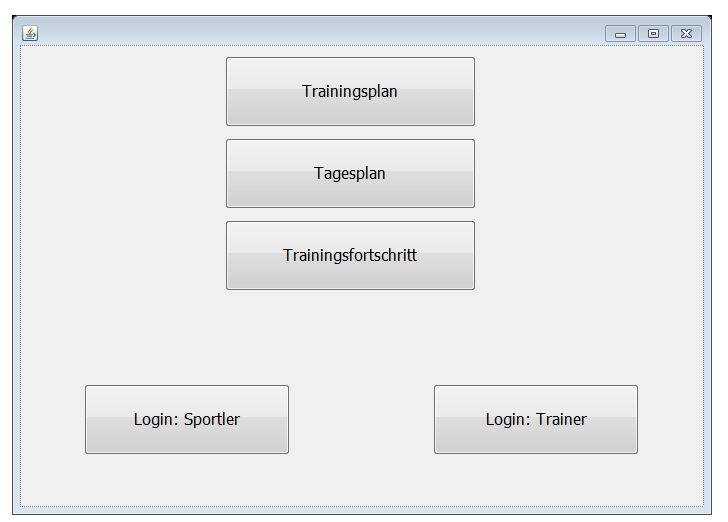
\includegraphics[width=0.75\hsize]{./menu.jpg}
 \end{center}
\caption[Hauptmenü]{\label{haupt}Hauptmenü}
\end{figure}

Abbildung \ref{haupt} zeigt das Hauptmenü. Dieses Menü enthält fünf Buttons, welche jeweils zu einer Funktion des Programmes führt. Den gesamten Trainingsplan (Abb. \ref{planAll}), den Tagesplan (Abb. \ref{planDay}) und den Trainingsfortschritt (Abb. \ref{fortschritt}) kann man sich ohne Eingabe eines Passwortes anschauen. Um die Trainingsergebnisse einzutragen (Abb. \ref{sportlerView}) oder den Trainingsplan zu ändern (Abb. \ref{trainerView}) ist ein Passwort nötig.

\begin{figure}[H]
\begin{center}
 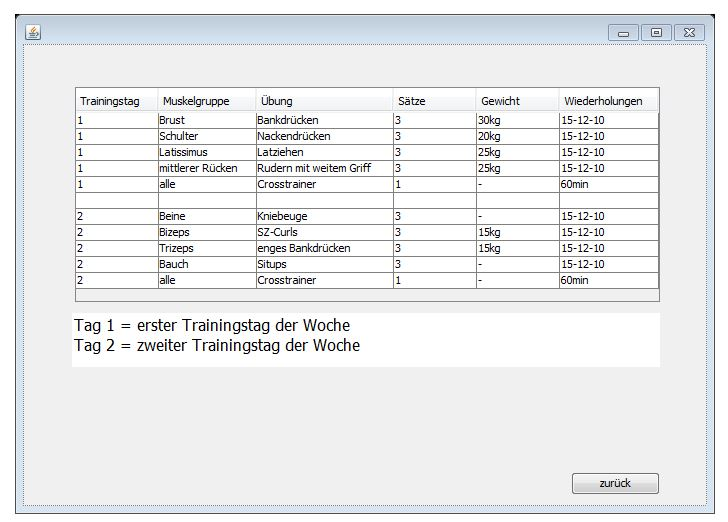
\includegraphics[width=0.75\hsize]{./trainingsplanView.jpg}
 \end{center}
\caption[Hauptmenü]{\label{planAll}gesamter Trainingsplan}
\end{figure}
Wie im vorangehenden Abschnitt erwähnt, erhält der Benutzer über die ersten drei Funktionen lesenden Zugriff auf die Daten der Smartcard. Ein Beispiel für einen Trainingsplan ist in Abbildung \ref{planAll} zu sehen. Dieser enthält außer der Übersicht über die Übungen noch ein Textfeld für spezielle Anweisungen des Trainers.
\begin{figure}[H]
\begin{center}
 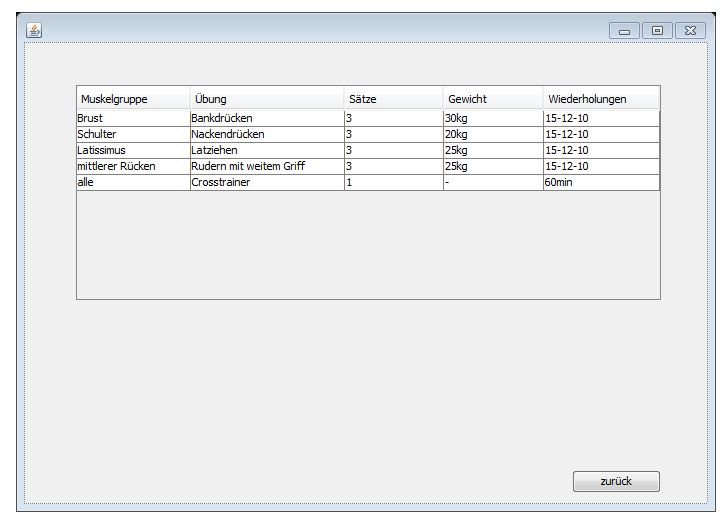
\includegraphics[width=0.75\hsize]{./tagesplanView.jpg}
 \end{center}
\caption[Trainingsplan für den aktuellen Tag]{\label{planDay}Trainingsplan für den aktuellen Tag}
\end{figure}
Im aktuellen Tagesplan (Abb. \ref{planDay}) sind die jeweiligen Übungen abgebildet.
\begin{figure}[H]
\begin{center}
 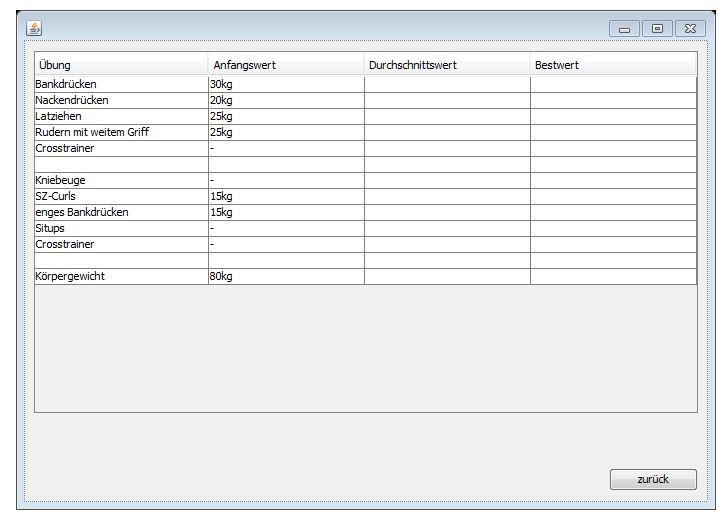
\includegraphics[width=0.75\hsize]{./fortschritt.jpg}
 \end{center}
\caption[Anzeige des Trainingsfortschrites]{\label{fortschritt}Anzeige des Trainingsfortschrites}
\end{figure}
Mithilfe der Trainingsfortschrittanzeige (Abb. \ref{fortschritt}) erhält der Sportler Auskunft über die Ausgangswerte seines derzeitigen Trainingsplanes, den Durchschnitt und seine Höchstleistung bei den entsprechenden Übungen. Weiterhin erhält er eine Info über seinen Gewichtsverlauf.
\begin{figure}[H]
\begin{center}
 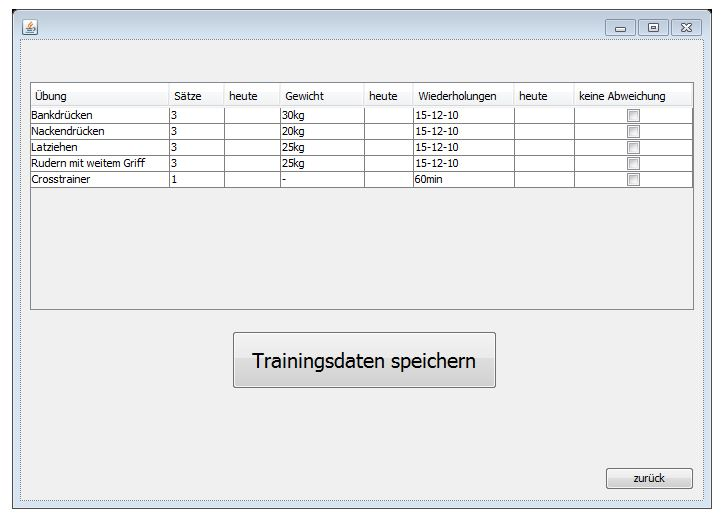
\includegraphics[width=0.75\hsize]{./sportlerView.jpg}
 \end{center}
\caption[Eingabe der Trainingsdaten]{\label{sportlerView}Eingabe der Trainingsdaten}
\end{figure}
Wenn man sich als Sportler eingeloggt hat, gelangt man zur Eingabe der Trainingsdaten (Abb. \ref{sportlerView}). Diese kann man alle manuell oder automatisch, per Checkbox ( Grundtrainingsdaten für die jeweiligen Übung), eintragen.


\begin{figure}[htb]
\begin{center}
 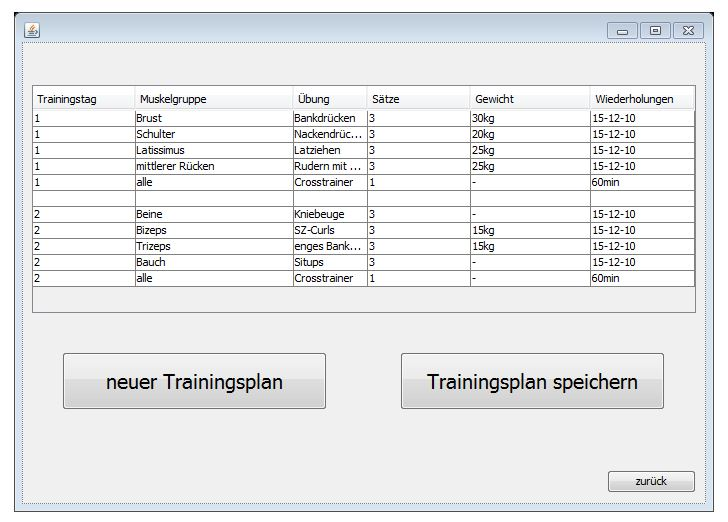
\includegraphics[width=0.75\hsize]{./trainerView.jpg}
 \end{center}
\caption[Erstellung und Änderung eines Trainingsplanes]{\label{trainerView}Erstellung und Änderung eines Trainingsplanes}
\end{figure}
In der Ansicht für den Trainer  (Abb. \ref{trainerView}), ist es möglich den Trainingsplan zu ändern bzw. einen neuen Plan anzulegen. Weiterhin existiert in jeder Unterfunktion des Hauptmenüs ein Zurück-Button, mit welchem man wieder ins Hauptmenü gelangt.

\section{Oncard}
%datenhaltung
%Logik für Datenzusammenhänge
Die Smartcard hält folgende Daten vor:
\begin{itemize}
\item Benutzerdaten bestehend aus Benutzerart und das gehashte Passwort
\item Trainingspläne
\item Trainingsfortschritt, welcher nach Benutzereingaben automatisch aktualisiert wird
\end{itemize}
%wegen geringem Speicherplatz alte Daten löschen oder bei Abruf vom trainer löschen

Die Auswertung von Anfragen und den überlieferten Daten sowie die Logik zur Aktualisierung des Trainingsfortschritts befindet sich ebenfalls auf der Smartcard.


\section{Offcard}
%Oberfläche
%Logik zur Oberfläche
Zum Offcard Programm zählt neben der GUI die dazugehörige Logik zum Abruf, senden und anzeigen der Daten.\\



\section{Aufgabenteilung}

\begin{itemize}
\item{GUI:} Michael Reher
\item{Offcard:} Marcel Kirbst
\item{Oncard:} Kurt Junghanns und Michael Reher
\end{itemize}

Abgabe ist der 11.7.2014.


%% So fügt man eine Vektorgrafik als PDF ein: (siehe Quellcode dieses Dokuments)

%\begin{figure}[htb]
%\begin{center}
% \includegraphics[width=1\hsize]{./Zeichnungen/IPv4NAT.pdf}
% \end{center}
%\caption[Beispielhafte Standardkonfiguration eines Internetanschlu\ss{} mit NAT, Quelle: Autor, verwendete Symbole unterliegen der
%GPL]{\label{stdinet}Beispielhafte Standardkonfiguration eines Internetanschlu\ss{}.}
%\end{figure}


\newpage
\pagenumbering{Roman}
\setcounter{page}{5} 


%Glossar
%\newpage
%\section*{Glossar}
%\addcontentsline{toc}{chapter}{Glossar}
%\begin{description}
%\item[Eclipse] kostenfreie auf Java basierende IDE
%\end{description}

\newpage
\thispagestyle{empty}
\begin{center}
\Large{Hochschule für Technik, Wirtschaft und Kultur\\
Fakultät Informatik, Mathematik und Naturwissenschaften }\\
\end{center}

\begin{verbatim}






\end{verbatim}

\begin{center}
\textbf{\LARGE{Eidesstattliche Versicherung}}
\end{center}
\begin{verbatim}


\end{verbatim}

\begin{flushleft}
Wir erklären hiermit, dass wir diese Projektdokumentation selbstständig ohne Hilfe Dritter und ohne Benutzung anderer als der angegebenen Quellen und Hilfsmittel verfasst haben. Alle den benutzten Quellen wörtlich oder sinngemäß entnommenen Stellen sind als solche einzeln kenntlich gemacht.

Diese Arbeit ist bislang keiner anderen Prüfungsbehörde vorgelegt und auch nicht veröffentlicht worden.

Wir sind uns bewusst, dass eine falsche Erklärung rechtliche Folgen haben wird. 
\begin{verbatim}







\end{verbatim}
Leipzig, 11.7.2014, Marcel Kirbst
\hrule width .6\hsize\ \\
Leipzig, 11.7.2014, Kurt Junghanns
\hrule width .6\hsize\ \\
Leipzig, 11.7.2014, Michael Reher
\hrule width .6\hsize\ \\
Ort, Datum, Unterschrift
\end{flushleft}

\end{document}